\documentclass[11pt,letterpaper]{article}
\usepackage[top=1in,bottom=1in,left=1in,right=1in]{geometry}
\usepackage{natbib}      % http://merkel.zoneo.net/Latex/natbib.php
\usepackage{palatino}
\bibpunct{(}{)}{;}{a}{,}{,}
\usepackage{chngpage}
\usepackage{stmaryrd}
\usepackage{amssymb}
\usepackage{amsmath}
\usepackage{graphicx}
\usepackage{lscape}
\usepackage{subfigure}
\usepackage[usenames,dvipsnames]{color}
\definecolor{myblue}{rgb}{0,0.1,0.6}
\definecolor{mygreen}{rgb}{0,0.3,0.1}
\usepackage[colorlinks=true,linkcolor=black,citecolor=mygreen,urlcolor=myblue]{hyperref}

\newcommand{\bocomment}[1]{\textcolor{Bittersweet}{[#1 -BTO]}}

\newenvironment{itemizesquish}{\begin{list}{\labelitemi}{\setlength{\itemsep}{0em}\setlength{\labelwidth}{0.5em}\setlength{\leftmargin}{\labelwidth}\addtolength{\leftmargin}{\labelsep}}}{\end{list}}
\newcommand{\ignore}[1]{}
\newcommand{\transpose}{^\mathsf{T}}
\newcommand{\inner}[1]{\langle #1 \rangle}
\newcommand{\smallsec}[1]{\noindent \textbf{#1\ }}

\title{
  Model model model
}

\author{
Brendan O'Connor, Sam Thomson
}

%\date{December 9, 2009}

\begin{document}
\maketitle

\textbf{Data.} Every tuple has one \emph{trigger word} $w^{(h)}$ (a.k.a.~event head, or target word), and then one or more \emph{argument words} $w$.  (Perhaps single-words, perhaps phrases...)  Each argument also has, not just the word, but the \emph{syntactic path} $p$ between the argword and the triggerword.  (Perhaps including the POS at each end... the idea is to represent the syntactic configuration of the tuple, or in particular, just the syntactic relationship between the argument and the trigger.  Or could just say, whether is on left or right (like Lang/Lapata ``argument key''), etc.)

Let $a=1,2,..$ index the arguments within one tuple.  $a$ is meaningless to compare between tuples.  Thus a tuple $i$ (for $i=1..N$ tuples in the corpus) looks like:

\[ (w^{(h)}_i, [(w_{i,a}, p_{i,a})]_{a=1..A_i}) \]

where $A_i$ means the number of arguments in tuple $i$, say 1 or 2 or 3 or so.

\section{First model}

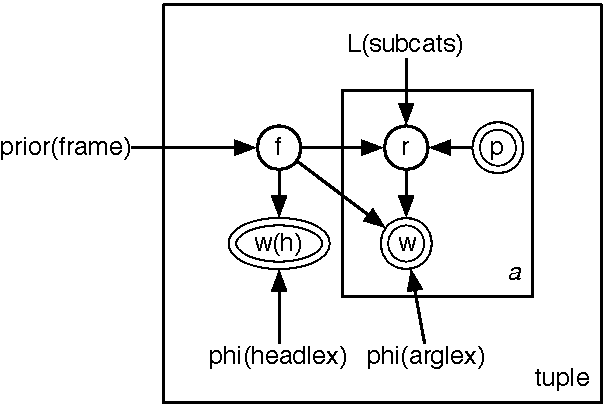
\includegraphics[width=2.5in]{diagram}

Variables in one tuple.  Leaving out $i$ subscripts

\begin{itemizesquish}
  \item $p$: syntactic path between trigger and argument word.  (related to Cheung's $dep_i$)
  \item $f$: frametype of the being-evoked frame.
  \item $r_a$: role being used for the argument (a.k.a.~frame element).
\end{itemizesquish}

To support a multinomial approach, let $f$ and $r_a$ be integer IDs.
There are $F$ possible frames ($f \in 1..F$), and for each frame, $R_f$ different roles.  (The roles within each frame are totally different and not comparable.  Identify just with integer IDs, $r_a \in 1..R_f$.)

Global parameters -- the frame system:

\begin{itemizesquish}
  \item $prior^{(frame})$: prior over the $F$ frames.
  \item $L^{(subcats)}$: the syntax-role linkage system.  For a given frame, it says which roles appear under which syntactic paths.  (Note the real notion of a subcat frame parameterizes multiple arguments at once.  The diagram here imposes a potentially problematic independence assumption.)
  \item $\phi^{(headlex)}$: the soft lexicon for what trigger words you expect to see for a frame.

  \item $\phi^{(arglex)}$: the soft lexicon for what argument words you expect to see for a particular role.  (or call it a frame-role combination, if you're really literally going by roles being integer IDs. this is why both $f$ and $r$ have to be parents in the DAG)
\end{itemizesquish}

(Convention: $\phi$ parameterizes distributions on words or word-like things.  
Maybe it's not words we want to generate, but rather (lemma,POS) pairs.)

There are lots of ways to stack this all together.  Here is one.

\textbf{Dirichlet-Multinomial model.}

Number of wordtypes $V$.  Fix $F$, every $R_f$.  All $\alpha$ are scalars (with diffuse priors)

\begin{itemizesquish}
  \item Each $\phi^{(headlex)}_f \sim Dir(V, \alpha^{(headlex)})$ and $\phi^{(arglex)}_{f,r}$ $\sim Dir(V, \alpha^{(arglex)})$
  \item For each $f$ and each $p$, $L_{f,p} \sim Dir(R_f, \alpha^{(L)})$
\end{itemizesquish}

To generate a tuple:

\begin{itemizesquish}
  \item $f \sim prior^{(frame)}$
  \item $w^{(h)} \sim \phi^{(h)}_f$
  \item For each $a$,
  \begin{itemizesquish}
    \item $r_a \sim L_{f,p}$
    \item $w_a \sim \phi^{(headlex)}_{f,r_a}$
  \end{itemizesquish}
\end{itemizesquish}

Training is really easy with collapsed Gibbs sampling.

Want to make $R_f$ nonparametric since it's a lot of hyperparameters to fix.
This is also a simple extension of the Gibbs sampler (go to CRP), though a tiny bit
harder to implement.

\textbf{Training with collapsed Gibbs sampling.}
Count ratios for generation probabilities (add pseudocounts to get CGS updates) are as follows.

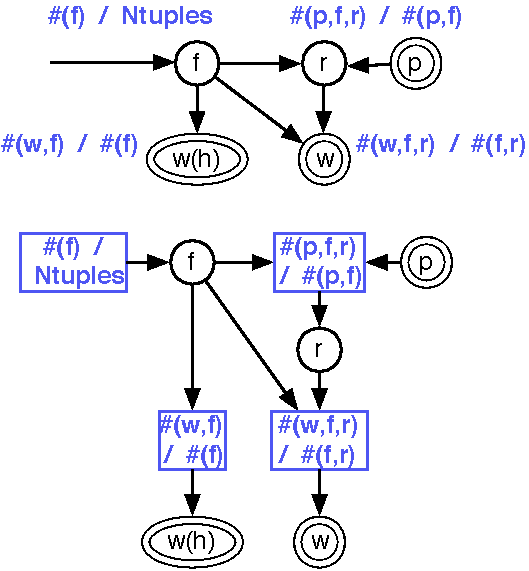
\includegraphics[width=3in]{cgs_ratios.pdf}


\section{Next model}

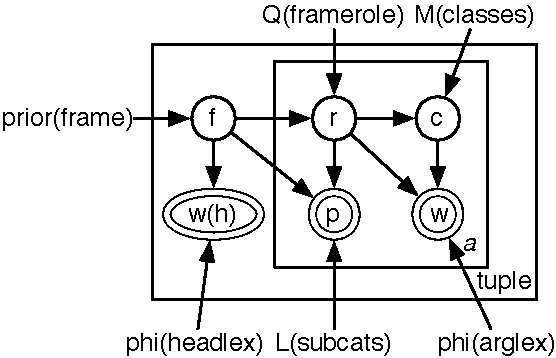
\includegraphics[width=3in]{diagram2}

% \bibliographystyle{plainnat}
% \bibliography{newbib}
\end{document}
